\subsection*{Метрики качества классификации.}

\subsubsection*{Доля верных ответов}

Итак, предполагаем, что у нашей модели есть 2 состояния: она предсказала неправильно или предсказала, но уже правильно.

Посчитаем количество объектов, на которых модель предсказала корректно:
\[
accuracy(a, X) = \frac{1}{\ell}\sum_{i=1}^\ell [a(x_i) = y_i]
\]

Эта штука называется долей верных ответов, и живые будут завидовать мёртвым, если вы где"=нибудь назовёте это точностью. Не переводите это как точность.

\subsubsection*{Confusion Matrix}

Проще показать, нежели пытаться описать, что это такое.

\begin{figure}[H]
    \centering
    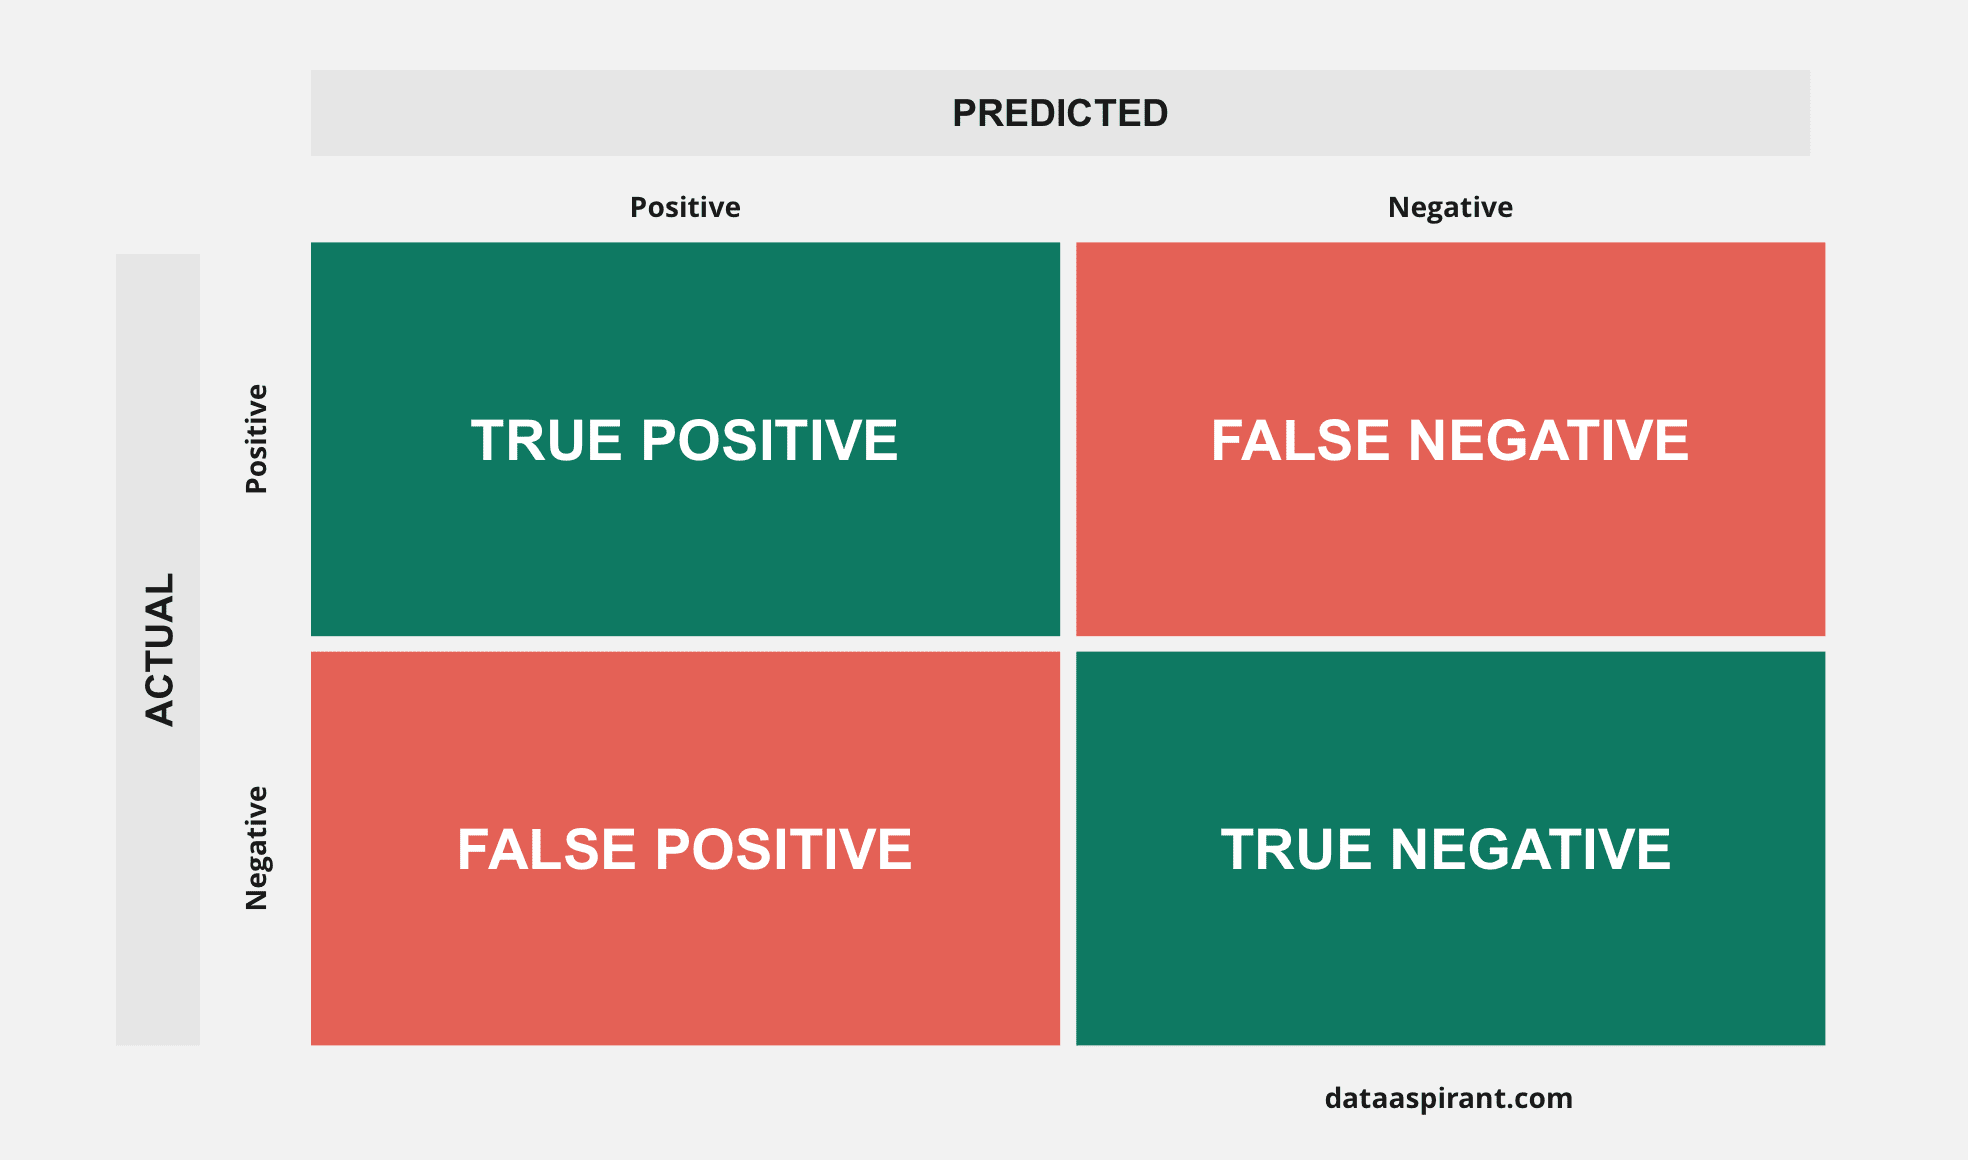
\includegraphics[width=0.9\linewidth]{media/conf_matr.png}
\end{figure}

Давайте теперь разбираться:
\begin{enumerate}
    \item \texttt{True Positive} "--- модель предсказала +1, реальный ответ +1;
    \item \texttt{False Negative} "--- модель предсказала -1, реальный ответ +1;
    \item \texttt{False Positive} "--- модель предсказала +1, реальный ответ -1;
    \item \texttt{True Negative} "--- модель предсказала -1, реальный ответ -1.
\end{enumerate}

Эта матрица сама по себе является метрикой, но помимо этого из неё вытекают базовые понятия для классификации, без которых в наши дни никуда.

\subsubsection*{Precision, recall (точность, полнота)}

Вот \texttt{precision} "--- это уже настоящая точность, тут можно говорить без всяких проблем. Формула выглядит следующим образом:
\[
precision = \frac{TP}{TP + FP}
\]
Это можно проинтерпретировать так: насколько можно доверять модели, если она предсказывает +1.

\texttt{recall} отражает то, насколько модель охватила положительный класс (т.е. сколько раз она поставила метку +1 на реально положительных объектах, относительно общего количества положительных объектов):
\[
recall = \frac{TP}{TP + FN}
\]

\subsubsection*{F"=мера}

Хотелось бы каким"=то образом объединить \texttt{precision, recall} в одну метрику. Это нужно для того, чтобы через одну метрику смотреть на поведение модели по двум метрикам сразу.

Сделать это можно с помощью \texttt{F-score}:
\[
F = \frac{2~precision~recall}{precision~+~recall}
\]

В общем смысле эту метрику называют $F_1$, и она является частным случаем $F_\beta$:
\[
F_\beta = \frac{(1 + \beta^2)~precision~recall}{\beta^2~precision + recall}
\]

Можно показать, что при $\beta \rightarrow 0$ важнее становится точность, а при $\beta \rightarrow \infty$ "--- полнота.

Метрик бывает, конечно, больше, но на данном этапе рассуждений можем остановиться пока на этих.